\section{Experiments \& Results}\label{sec:methodology}
This section outlines the experimental design used to identify the top-$n$ models to be used in our stacking ensemble.
We first describe the prequisite data preparation for all our experiments, followed by a description of the hardware and software used.
Next, we outline the design of our initial experiment, aimed at providing a preliminary assesment of the models selected in Section~\ref{sec:model_selection}.
Following this, we present and discuss the results of this experiment.
We then describe the design of our main experiment, where we use our hyperparameter tuning framework to identify the top-$n$ models.
The results are then presented and discussed the results of this experiment.
Finally, we use the identified models to construct a stacking ensemble, which is then evaluated and compared to the individual models.

\subsection{Data Preparation}\label{sec:data-preparation}
The first step in our methodology is to prepare the datasets for model training and evaluation.
As mentioned in Section~\ref{sec:data-overview}, the data used in this study was obtained from \gls{nasa}'s \gls{pds} and consists of \gls{ccs} data and major oxide compositions for various samples.

The initial five shots from each sample are excluded because they are usually contaminated by dust covering the sample, which is cleared away by the shock waves produced by the laser \cite{cleggRecalibrationMarsScience2017}.
The remaining 45 shots from each location are then averaged, yielding a single spectrum $s$ per location $l$ in the \texttt{Averaged Intensity Tensor} (Tensor \ref{matrix:averaged_intensity}), resulting in a total of five spectra for each sample.

At this stage, the data still contains noise at the edges of the spectrometers.
These edges correspond to the boundaries of the three spectrometers, which collectively cover the \gls{uv}, \gls{vio}, and \gls{vnir} light spectra.
The noisy edge ranges are as follows: 240.811-246.635 nm, 338.457-340.797 nm, 382.138-387.859 nm, 473.184-492.427 nm, and 849-905.574 nm.
In addition to being noisy regions, these regions do not contain any useful information related to each of the major oxides.
Consequently, these regions are masked by zeroing out the values, rather than removing them, as they represent meaningful variation in the data~\cite{cleggRecalibrationMarsScience2017}.

Additionally, as a result of the aforementioned preprocessing applied to the raw \gls{libs} data, negative values are present in the \gls{ccs} data.
These negative values are not physically meaningful, since you cannot have negative light intensity \cite{p9_paper}.
Similar to the noisy edges, these negative values are also masked by zeroing out the values.

We transpose the data so that each row represents a location and each column represents a wavelength feature.
Each location is now represented as a vector of wavelengths, with the corresponding average intensity values for each wavelength.
These vectors are then concatenated to form a tensor, giving us the full \texttt{Averaged Intensity Tensor}.

For each sample, we have a corresponding set of major oxide compositions in weight percentage (wt\%).
These compositions are used as the target labels for the machine learning models.
An excerpt of this data is shown in Table \ref{tab:composition_data_example}.
While the \textit{Target}, \textit{Spectrum Name}, and \textit{Sample Names} are part of the dataset, our analysis focuses primarily on the \textit{Sample Names}.
The concentrations of the eight oxides \ce{SiO2}, \ce{TiO2}, \ce{Al2O3}, \ce{FeO_T}, \ce{MnO}, \ce{MgO}, \ce{CaO}, \ce{Na2O}, and \ce{K2O} represent the expected values for these oxides in the sample, serving as our ground truth. The \textit{MOC total} is not utilized in this study.

\begin{table*}
\centering
\caption{Excerpt from the composition dataset (from \citet{p9_paper}).}
\begin{tabular}{lllllllllllll}
\toprule
     Target & Spectrum Name & Sample Name & \ce{SiO2} & \ce{TiO2} & \ce{Al2O3} & \ce{FeO_T} & \ce{MnO} & \ce{MgO} & \ce{CaO} & \ce{Na2O} & \ce{K2O} & \ce{MOC total} \\
\midrule
AGV2 & AGV2 & AGV2 & 59.3 & 1.05 & 16.91 & 6.02 & 0.099 & 1.79 & 5.2 & 4.19 & 2.88 & 97.44 \\
BCR-2 & BCR2 & BCR2 & 54.1 & 2.26 & 13.5 & 12.42 & 0.2 & 3.59 & 7.12 & 3.16 & 1.79 & 98.14 \\
$\vdots$ & $\vdots$ & $\vdots$ & $\vdots$ & $\vdots$ & $\vdots$ & $\vdots$ & $\vdots$ & $\vdots$ & $\vdots$ & $\vdots$ & $\vdots$ & $\vdots$ \\
TB & --- & --- & 60.23 & 0.93 & 20.64 & 11.6387 & 0.052 & 1.93 & 0.000031 & 1.32 & 3.87 & 100.610731 \\
    TB2 & --- & --- & 60.4 & 0.93 & 20.5 & 11.6536 & 0.047 & 1.86 & 0.2 & 1.29 & 3.86 & 100.7406 \\
\bottomrule
\end{tabular}
\label{tab:composition_data_example}
\end{table*}

The major oxide weight percentages are appended to the matrix of spectral data, forming the final dataset.
This dataset is shown in Table~\ref{tab:final_dataset_example}.
The \textit{Target} column corresponds to the sample name, while the \textit{ID} column contains the unique identifier for each location.

\begin{table*}
\centering
\caption{Excerpt from the final dataset (values have been rounded to two decimal places for brevity).}
\footnotesize
\begin{tabular}{llllllllllllllllllllll}
\toprule
    240.81   & $\cdots$     & 425.82    & 425.87   & $\cdots$ & 905.57  & \ce{SiO2} & \ce{TiO2} & \ce{Al2O3} & \ce{FeO_T} & \ce{MgO} & \ce{CaO} & \ce{Na2O} & \ce{K2O} & Target     & ID \\
\midrule
	0        & $\cdots$     & 1.53e+10 & 1.62e+10 & $\cdots$ & 0        & 56.13     & 0.69 & 17.69 & 5.86 & 3.85 & 7.07 & 3.32 & 1.44 & jsc1421     & jsc1421\_2013\_09\_12\_211002\_ccs \\
	0        & $\cdots$     & 1.28e+10 & 1.30e+10 & $\cdots$ & 0        & 56.13     & 0.69 & 17.69 & 5.86 & 3.85 & 7.07 & 3.32 & 1.44 & jsc1421     & jsc1421\_2013\_09\_12\_211143\_ccs \\
    0        & $\cdots$     & 1.87e+10 & 1.83e+10 & $\cdots$ & 0        & 56.13     & 0.69 & 17.69 & 5.86 & 3.85 & 7.07 & 3.32 & 1.44 & jsc1421     & jsc1421\_2013\_09\_12\_210628\_ccs \\
    0        & $\cdots$     & 1.77e+10 & 1.78e+10 & $\cdots$ & 0        & 56.13     & 0.69 & 17.69 & 5.86 & 3.85 & 7.07 & 3.32 & 1.44 & jsc1421     & jsc1421\_2013\_09\_12\_210415\_ccs \\
    0        & $\cdots$     & 1.75e+10 & 1.79e+10 & $\cdots$ & 0        & 56.13     & 0.69 & 17.69 & 5.86 & 3.85 & 7.07 & 3.32 & 1.44 & jsc1421     & jsc1421\_2013\_09\_12\_210811\_ccs \\
    0        & $\cdots$     & 5.52e+10 & 3.74e+10 & $\cdots$ & 0        & 57.60     & 0.78 & 26.60 & 2.73 & 0.70 & 0.01 & 0.38 & 7.10 & pg7         & pg7\_2013\_11\_07\_161903\_ccs \\
    0        & $\cdots$     & 5.09e+10 & 3.41e+10 & $\cdots$ & 0        & 57.60     & 0.78 & 26.60 & 2.73 & 0.70 & 0.01 & 0.38 & 7.10 & pg7         & pg7\_2013\_11\_07\_162038\_ccs \\
    0        & $\cdots$     & 5.99e+10 & 3.97e+10 & $\cdots$ & 0        & 57.60     & 0.78 & 26.60 & 2.73 & 0.70 & 0.01 & 0.38 & 7.10 & pg7         & pg7\_2013\_11\_07\_161422\_ccs \\
    0        & $\cdots$     & 5.22e+10 & 3.47e+10 & $\cdots$ & 0        & 57.60     & 0.78 & 26.60 & 2.73 & 0.70 & 0.01 & 0.38 & 7.10 & pg7         & pg7\_2013\_11\_07\_161735\_ccs \\
    0        & $\cdots$     & 5.29e+10 & 3.62e+10 & $\cdots$ & 0        & 57.60     & 0.78 & 26.60 & 2.73 & 0.70 & 0.01 & 0.38 & 7.10 & pg7         & pg7\_2013\_11\_07\_161552\_ccs \\
	$\vdots$ & $\cdots$ & $\vdots$ & $\vdots$ & $\cdots$ & $\vdots$ & $\vdots$ & $\vdots$ & $\vdots$ & $\vdots$ & $\vdots$ & $\vdots$ & $\vdots$ & $\vdots$ & $\vdots$ & $\vdots$ \\
\midrule
\end{tabular}
\label{tab:final_dataset_example}
\end{table*}
\subsection{Experimental Setup}
Experiments were conducted on a machine equipped with an Intel Xeon Gold 6242 CPU, featuring 16 cores and 32 threads.
The CPU has a base clock speed of 2.80 GHz and a maximum turbo frequency of 3.90 GHz.
The system has 64 GB of RAM and runs on Ubuntu 22.04.2 LTS.
Models were implemented using Python 3.10.11.
The primary libraries used were Scikit-learn 1.4.2, XGBoost 2.0.3, Torch 2.2.2, NumPy 1.26.4, Pandas 2.2.1, Keras 3.2.1 and Optuna 3.6.1.
Additionally, all experiments were run using the hyperparameter optimization tool described in Section~\ref{subsec:hyperparameter_tuning_tool}. % TODO: Add correct ref once other PR is in
\subsection{Design for Initial Experiment}\label{sec:initial-experiment}
As described in Section~\ref{sec:proposed_approach}, we conducted a series of initial experiments to evaluate the performance of various machine learning models on the prediction of major oxide compositions from our \gls{libs} dataset.
These experiments aimed to provide a preliminary assessment of the models' performance, allowing us to identify the most promising models for further evaluation and inclusion in our stacking ensemble.
All models were trained on the same preprocessed data using the Norm 3 preprocessing method described in Section~\ref{sec:norm3}.
This ensured that the models' performance could be evaluated under consistent and comparable conditions.

All models were trained using our data partitioning and cross-validation strategy, as described in Section~\ref{subsec:validation_testing_procedures}. 
To ensure as fair of a comparison between models as possible, all models were trained using as many default hyperparameters as possible, and those hyperparameters that did not have default options were selected based on values found in the literature.
However, due to the nature of the neural network models' architecture, some extra time was spent on tuning the models to ensure a fair comparison.
This included using batch normalization for the \gls{cnn} model, as early assesments showed that this was necessary to produce reasonable results.
Finally, we evaluated each model once per oxide given the selected configuration of hyperparameters. 
As stated, the goal of this experiment was merely to get an initial indication of the performance of the models.

The hyperparameters used for the models in the initial experiment can be found in the Appendix~\ref{subsec:initial_experiment_hyperparameters}.
\subsection{Initial Results}
Table~\ref{tab:init_results} presents the results of the initial experiments, including the \gls{rmsep}, \gls{rmsecv}, standard deviation, and standard deviation of cross-validation prediction errors for each model across all oxides.
The means of each metric are also provided to give an overall indication of the models' performance.
Furthermore, we present an overview of these mean values in Figure~\ref{fig:init_results_rmses} to facilitate a visual comparison of the models' general performance.

The results indicate that the gradient boosting models, \gls{xgboost}, \gls{gbr}, and \gls{ngboost}, consistently perform well across all oxides, with \gls{xgboost} generally outperforming the other two gradient boosting models.
Interestingly, \gls{gbr} has the lowest \gls{rmsep}, while \gls{xgboost} achieves the lowest \gls{rmsecv}, suggesting that the regularization in \gls{xgboost} may improve the model's generalizability.
These models exhibit both low mean \gls{rmsep} and \gls{rmsecv} values, indicating high accuracy, as well as low standard deviation values, underscoring their robustness.
\gls{svr} is also among the top-performing models, with mean \gls{rmsep} and \gls{rmsecv} values close to those of \gls{xgboost} and low standard deviation values.

While usually outperformed by gradient boosting models and \gls{svr}, the other ensemble models, \gls{rf} and \gls{etr}, also exhibit good performance.
The \gls{pls}, ridge, \gls{lasso}, and \gls{enet} models typically seem to perform worse than the other models, with higher mean \gls{rmsep} and \gls{rmsecv} values and higher standard deviation values.
We observe that \gls{enet} performs between ridge and \gls{lasso} in terms of both error and standard deviation, which aligns with expectations since \gls{enet} combines the regularization techniques of both models.

The \gls{cnn} and \gls{ann} models perform the worst across all oxides, exhibiting the highest mean \gls{rmsep} and \gls{rmsecv} values, as well as the highest standard deviation values.
This poor performance is further highlighted in Table~\ref{tab:relative_performance}, which shows the relative performance of each model compared to the best-performing model, \gls{xgboost}.
The table also includes the difference in performance relative to the next best model, with \gls{xgboost} serving as the baseline for comparison, assigned a relative performance of 100\%.
From this table, it is evident that the \gls{cnn} and \gls{ann} models experience notable drops in performance compared to the top-performing models.
While deep learning models such as these have the theoretical potential to perform well with \gls{libs} data, given their ability to learn complex patterns and relationships, the relatively small size of our dataset may limit their efficacy.
Furthermore, achieving optimal performance with these models necessitates extensive tuning of both their architectures and hyperparameters, which involves exploring a vast space of potential configurations and design choices.
Although methods for systematic hyperparameter optimization, as detailed in Section~\ref{sec:optimization_framework}, could be employed, the associated computational cost would be prohibitively high.
Additionally, there are numerous architectural design decisions and advanced techniques that could potentially enhance model performance, but their inclusion would expand the scope of this study beyond feasible limits.
For these reasons, we decided to exclude the \gls{cnn} and \gls{ann} models from further experimentation.

Tables~\ref{tab:best_results} and \ref{tab:best_model_occurrences} list the best-performing model for each oxide and the frequency with which each model achieves top performance according to various metrics, respectively.
These tables are intended to provide an overview of model performance rather than to determine an overall 'winner by majority'.
Their purpose is to illustrate the general trends and behavior of different models across various metrics and oxides.
Although \gls{xgboost} and \gls{svr} appear the most frequently in Table~\ref{tab:best_model_occurrences}, this does not imply that they are the best models for every oxide.
For example, if one were to only consider the mean of the performance metrics, \gls{pls} would be considered among the worst performing models, as shown in Figure~\ref{fig:init_results_rmses}.
However, inspecting Table~\ref{tab:best_results} reveals that \gls{pls} exhibits the lowest \gls{rmsecv} and standard deviation of prediction errors for both \ce{MgO} and \ce{Na2O}.
This indicates that \gls{pls} is the most accurate and robust model for these oxides, underscoring the importance of evaluating model performance on a per-oxide basis, as discussed in Section~\ref{sec:proposed_approach}.
Moreover, for some oxides, multiple models perform similarly well, such as \gls{xgboost}, \gls{gbr}, and ridge for \ce{CaO}.
This observation suggests the potential benefit of leveraging the strengths of multiple models, provided they do not make similar types of errors, which warrants further investigation.

To summarize, the initial results indicate that gradient boosting models, particularly \gls{xgboost}, demonstrated the most consistent and accurate performance across all oxides.
\gls{svr} also performed well, with similar accuracy and robustness to the gradient boosting models.
In contrast, deep learning models such as \gls{cnn} and \gls{ann} underperformed, likely due to the small dataset size and insufficient tuning of their architectures and hyperparameters.
Inspecting the model performances per oxide revealed that the best model varied depending on the oxide, and several models performed well for each oxide.
This emphasizes the need for further evaluation of model performances on a per-oxide basis to identify suitable configurations for our stacking ensemble approach, which aims to leverage the strengths of multiple models.

\begin{figure*}
    \centering
    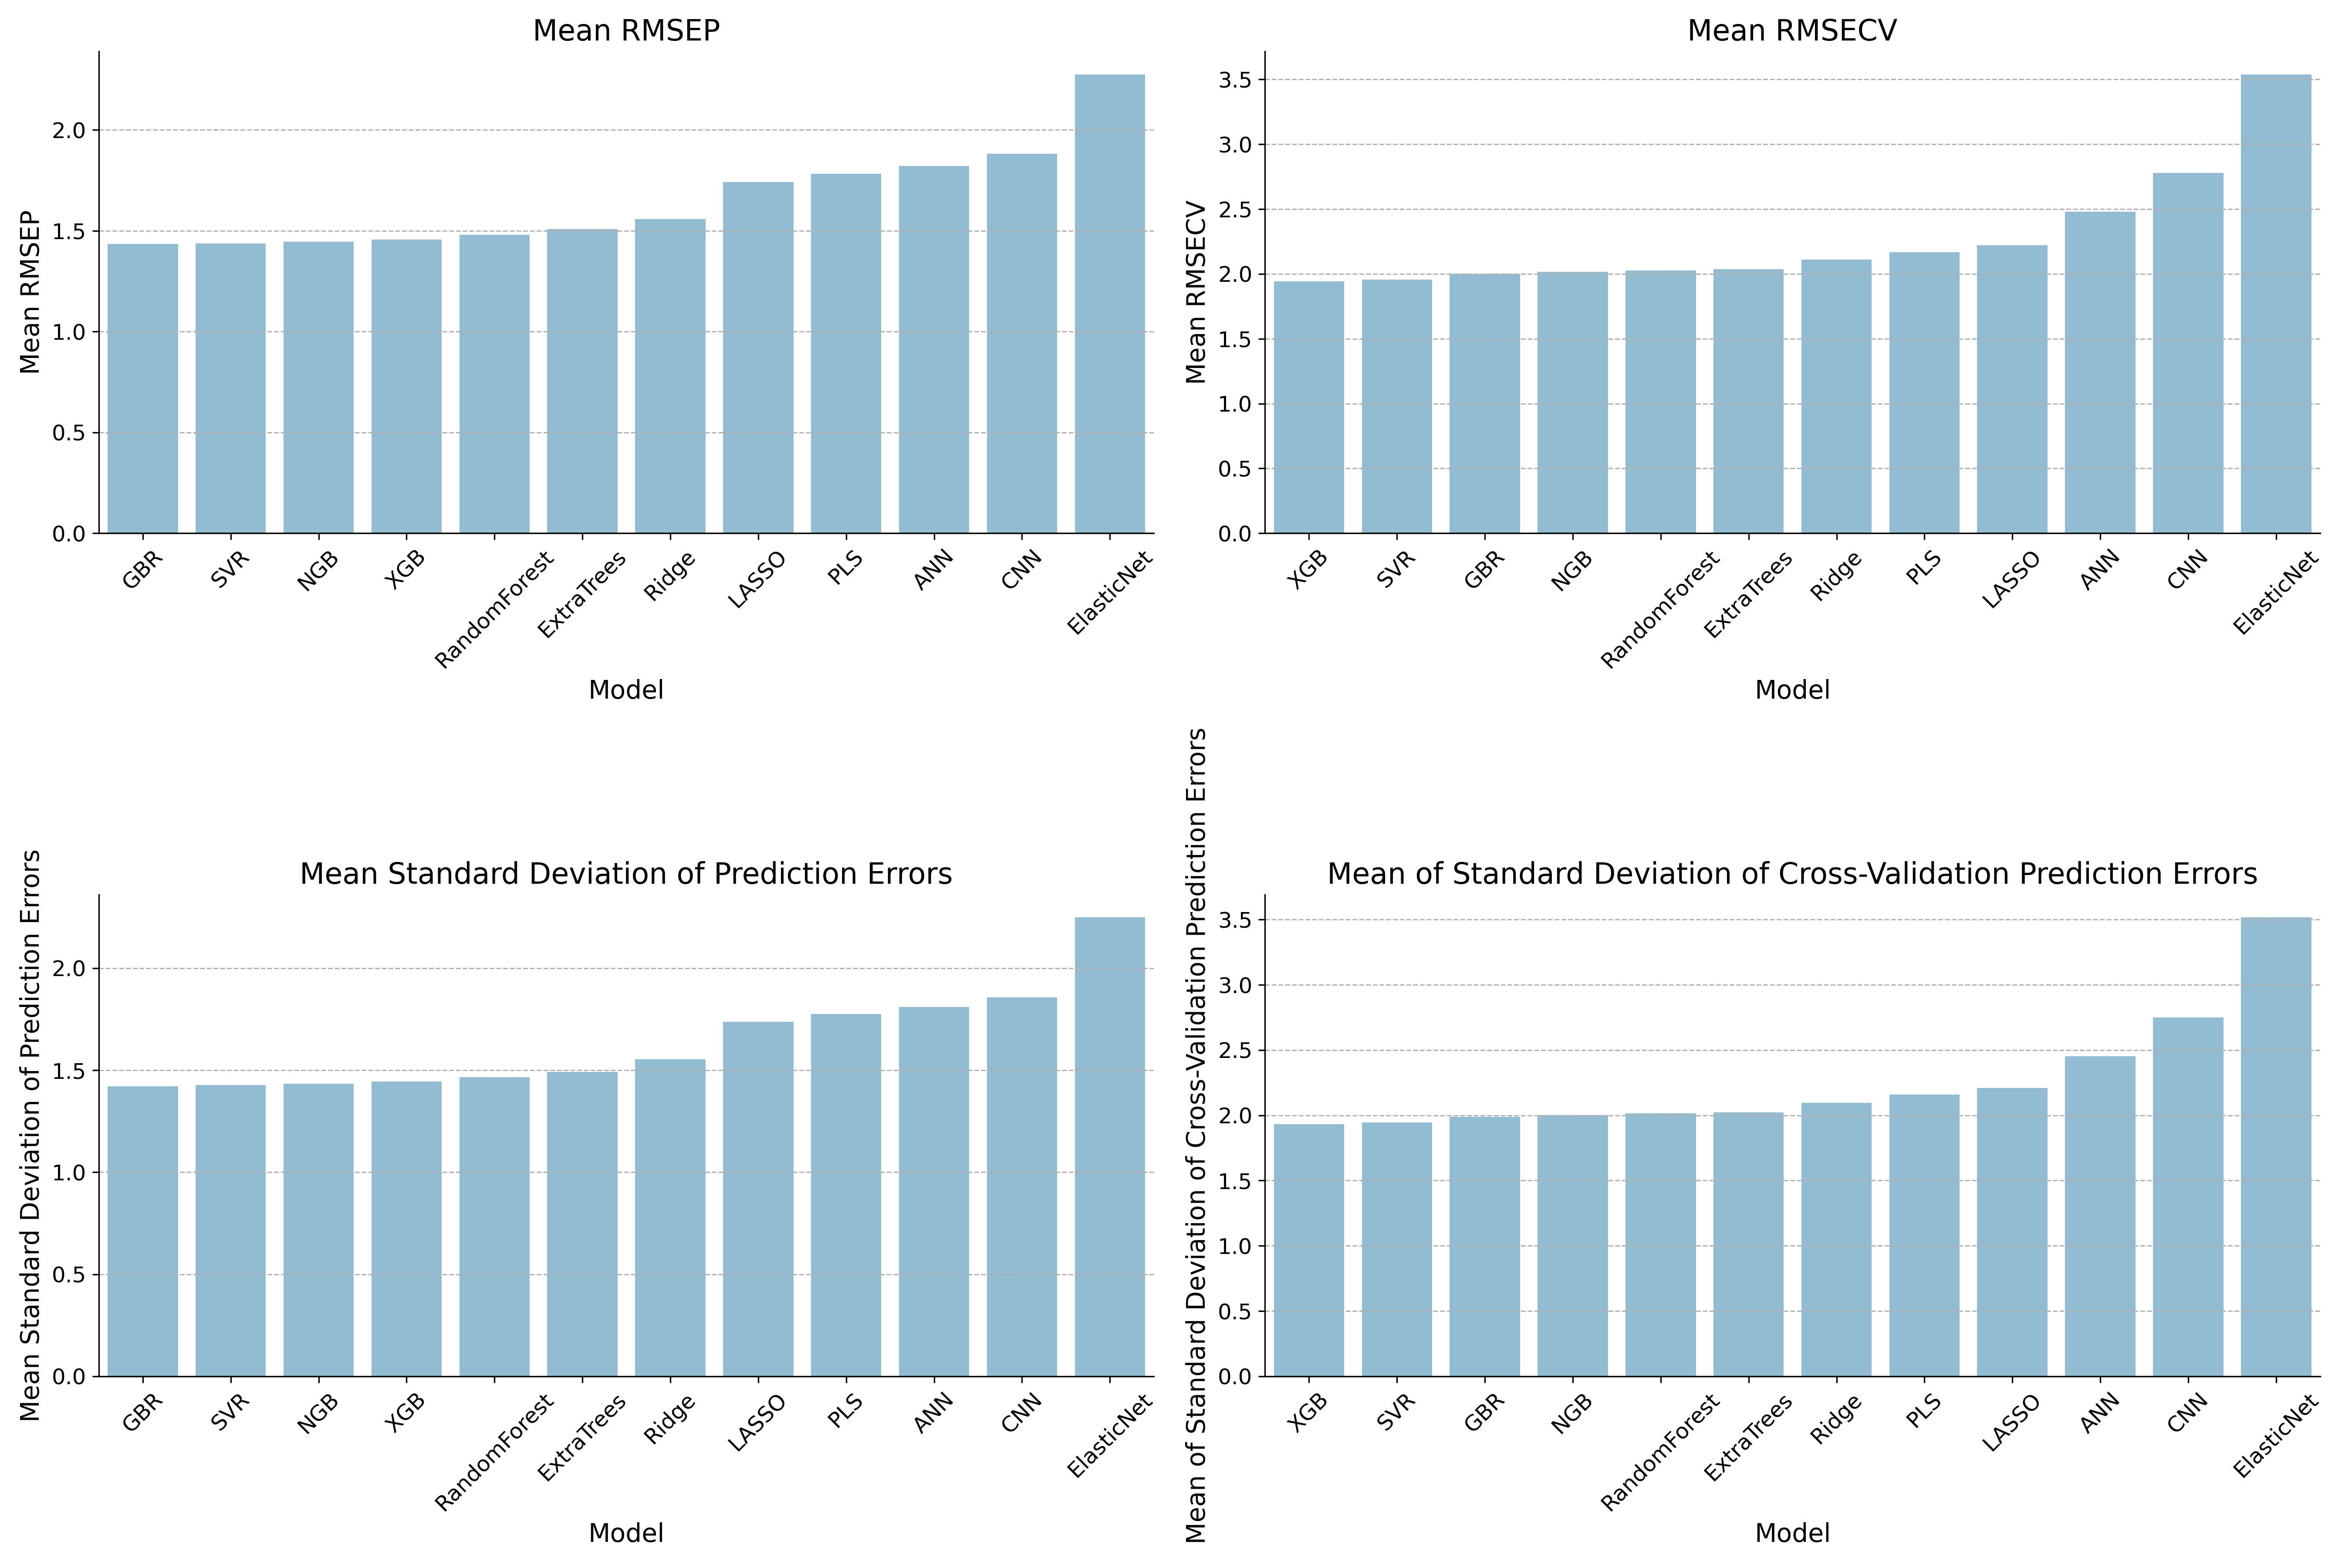
\includegraphics[width=\textwidth]{images/init_results_means.png}
    \caption{Mean \gls{rmsep}, \gls{rmsecv}, standard deviation of prediction errors, and standard deviation of cross-validation prediction errors for each model across all oxides.}
    \label{fig:init_results_rmses}
\end{figure*}

\begin{table}
\caption{Relative performance of each model compared to the best performing model, measured by normalized RMSECV and multiplied by 100 for percentage. A higher percentage indicates worse performance. The 'Diff. vs Prev.' column shows the difference in performance compared to the next best model, measured in percentage points.}
\begin{tabular}{lrr}
\toprule
Model & Relative Performance (\%) & Diff. vs Prev. \\
\midrule
XGB & 100.00 & - \\
SVR & 100.85 & 0.85 \\
GBR & 103.07 & 2.22 \\
NGB & 103.94 & 0.87 \\
RandomForest & 104.45 & 0.51 \\
ExtraTrees & 104.84 & 0.39 \\
Ridge & 105.04 & 0.20 \\
PLS & 111.66 & 6.61 \\
ElasticNet & 114.12 & 2.46 \\
LASSO & 114.30 & 0.19 \\
ANN & 127.82 & 13.52 \\
CNN & 143.18 & 15.36 \\
\bottomrule
\end{tabular}
\label{tab:relative_performance}
\end{table}

\begin{table*}[]
\centering
\caption{Initial results for the different models and metrics.}
\resizebox{1\textwidth}{!}{%
\begin{tabular}{l|cccc|cccc|cccc}
Model & \multicolumn{4}{c}{Ridge} & \multicolumn{4}{c}{\gls{lasso}} & \multicolumn{4}{c}{\gls{enet}} \\
Metric & \multicolumn{1}{c}{RMSEP} & \multicolumn{1}{c}{RMSECV} & \multicolumn{1}{c}{Std. dev.} & \multicolumn{1}{c}{Std. dev. CV} & \multicolumn{1}{c}{RMSEP} & \multicolumn{1}{c}{RMSECV} & \multicolumn{1}{c}{Std. dev.} & \multicolumn{1}{c}{Std. dev. CV} & \multicolumn{1}{c}{RMSEP} & \multicolumn{1}{c}{RMSECV} & \multicolumn{1}{c}{Std. dev.} & \multicolumn{1}{c}{Std. dev. CV} \\
\hline
$\ce{SiO2}$ & 4.104 & 5.004 & 4.108 & 5.005 & 4.412 & 5.431 & 4.417 & 5.437 & 4.412 & 5.431 & 4.417 & 5.437 \\
$\ce{TiO2}$ & 0.424 & 0.470 & 0.413 & 0.469 & 0.398 & 0.556 & 0.389 & 0.555 & 0.398 & 0.556 & 0.389 & 0.555 \\
$\ce{Al2O3}$ & 2.322 & 2.913 & 2.324 & 2.888 & 2.349 & 3.063 & 2.352 & 3.044 & 2.349 & 3.063 & 2.352 & 3.044 \\
$\ce{FeOT}$ & 2.068 & 3.173 & 2.070 & 3.122 & 2.236 & 3.490 & 2.238 & 3.440 & 2.236 & 3.490 & 2.238 & 3.440 \\
$\ce{MgO}$ & 1.150 & 1.509 & 1.152 & 1.492 & 1.267 & 1.682 & 1.249 & 1.661 & 1.267 & 1.682 & 1.249 & 1.661 \\
$\ce{CaO}$ & 1.844 & 1.485 & 1.833 & 1.478 & 1.963 & 1.554 & 1.962 & 1.549 & 1.963 & 1.554 & 1.962 & 1.549 \\
$\ce{Na2O}$ & 0.632 & 1.089 & 0.633 & 1.084 & 0.625 & 1.114 & 0.616 & 1.111 & 0.588 & 1.085 & 0.587 & 1.082 \\
$\ce{K2O}$ & 0.651 & 0.668 & 0.645 & 0.668 & 0.638 & 0.859 & 0.629 & 0.856 & 0.638 & 0.859 & 0.629 & 0.856 \\
\hline
Mean & 1.649 & 2.039 & 1.647 & 2.026 & 1.736 & 2.219 & 1.732 & 2.207 & 1.731 & 2.215 & 1.728 & 2.203 \\
\hline
Model & \multicolumn{4}{c}{\gls{pls}} & \multicolumn{4}{c}{\gls{svr}} & \multicolumn{4}{c}{\gls{rf}} \\
Metric & \multicolumn{1}{c}{RMSEP} & \multicolumn{1}{c}{RMSECV} & \multicolumn{1}{c}{Std. dev.} & \multicolumn{1}{c}{Std. dev. CV} & \multicolumn{1}{c}{RMSEP} & \multicolumn{1}{c}{RMSECV} & \multicolumn{1}{c}{Std. dev.} & \multicolumn{1}{c}{Std. dev. CV} & \multicolumn{1}{c}{RMSEP} & \multicolumn{1}{c}{RMSECV} & \multicolumn{1}{c}{Std. dev.} & \multicolumn{1}{c}{Std. dev. CV} \\
\hline
$\ce{SiO2}$ & 4.141 & 5.701 & 4.145 & 5.693 & 3.552 & 4.908 & 3.555 & 4.908 & 3.715 & 5.304 & 3.699 & 5.292 \\
$\ce{TiO2}$ & 0.452 & 0.531 & 0.441 & 0.530 & 0.461 & 0.463 & 0.455 & 0.462 & 0.331 & 0.427 & 0.321 & 0.425 \\
$\ce{Al2O3}$ & 2.073 & 3.322 & 2.061 & 3.302 & 1.931 & 2.700 & 1.934 & 2.693 & 2.076 & 2.443 & 2.079 & 2.433 \\
$\ce{FeOT}$ & 3.222 & 3.117 & 3.221 & 3.114 & 1.823 & 2.847 & 1.814 & 2.809 & 2.091 & 3.091 & 2.073 & 3.053 \\
$\ce{MgO}$ & 1.106 & 1.296 & 1.103 & 1.296 & 0.789 & 1.426 & 0.785 & 1.419 & 0.911 & 1.742 & 0.904 & 1.731 \\
$\ce{CaO}$ & 1.937 & 1.813 & 1.923 & 1.792 & 1.626 & 1.532 & 1.594 & 1.508 & 1.765 & 1.503 & 1.754 & 1.499 \\
$\ce{Na2O}$ & 0.545 & 0.908 & 0.536 & 0.906 & 0.742 & 1.096 & 0.725 & 1.086 & 0.420 & 1.028 & 0.421 & 1.023 \\
$\ce{K2O}$ & 0.774 & 0.650 & 0.772 & 0.646 & 0.567 & 0.690 & 0.555 & 0.689 & 0.524 & 0.681 & 0.476 & 0.676 \\
\hline
Mean & 1.781 & 2.167 & 1.775 & 2.160 & 1.436 & 1.958 & 1.427 & 1.947 & 1.479 & 2.027 & 1.466 & 2.017 \\
\hline
Model & \multicolumn{4}{c}{\gls{ngboost}} & \multicolumn{4}{c}{\gls{gbr}} & \multicolumn{4}{c}{\gls{xgboost}} \\
Metric & \multicolumn{1}{c}{RMSEP} & \multicolumn{1}{c}{RMSECV} & \multicolumn{1}{c}{Std. dev.} & \multicolumn{1}{c}{Std. dev. CV} & \multicolumn{1}{c}{RMSEP} & \multicolumn{1}{c}{RMSECV} & \multicolumn{1}{c}{Std. dev.} & \multicolumn{1}{c}{Std. dev. CV} & \multicolumn{1}{c}{RMSEP} & \multicolumn{1}{c}{RMSECV} & \multicolumn{1}{c}{Std. dev.} & \multicolumn{1}{c}{Std. dev. CV} \\
\hline
$\ce{SiO2}$ & 4.112 & 5.071 & 4.081 & 5.010 & 3.576 & 4.995 & 3.479 & 4.922 & 3.953 & 4.898 & 3.926 & 4.876 \\
$\ce{TiO2}$ & 0.340 & 0.433 & 0.333 & 0.430 & 0.474 & 0.449 & 0.473 & 0.446 & 0.334 & 0.437 & 0.328 & 0.436 \\
$\ce{Al2O3}$ & 1.931 & 2.291 & 1.933 & 2.282 & 1.894 & 2.518 & 1.891 & 2.511 & 1.912 & 2.198 & 1.913 & 2.193 \\
$\ce{FeOT}$ & 1.588 & 3.561 & 1.590 & 3.530 & 1.594 & 3.069 & 1.596 & 3.068 & 1.848 & 3.020 & 1.838 & 3.002 \\
$\ce{MgO}$ & 0.849 & 1.578 & 0.845 & 1.574 & 0.964 & 1.766 & 0.960 & 1.763 & 0.905 & 1.781 & 0.901 & 1.771 \\
$\ce{CaO}$ & 1.740 & 1.610 & 1.723 & 1.602 & 1.768 & 1.468 & 1.769 & 1.468 & 1.765 & 1.467 & 1.749 & 1.457 \\
$\ce{Na2O}$ & 0.416 & 0.921 & 0.415 & 0.916 & 0.481 & 1.130 & 0.481 & 1.123 & 0.387 & 1.071 & 0.387 & 1.062 \\
$\ce{K2O}$ & 0.582 & 0.675 & 0.545 & 0.673 & 0.727 & 0.609 & 0.719 & 0.610 & 0.547 & 0.658 & 0.511 & 0.657 \\
\hline
Mean & 1.445 & 2.017 & 1.433 & 2.002 & 1.435 & 2.001 & 1.421 & 1.989 & 1.456 & 1.941 & 1.444 & 1.932 \\
\hline
Model & \multicolumn{4}{c}{\gls{etr}} & \multicolumn{4}{c}{\gls{ann}} & \multicolumn{4}{c}{\gls{cnn}} \\
Metric & \multicolumn{1}{c}{RMSEP} & \multicolumn{1}{c}{RMSECV} & \multicolumn{1}{c}{Std. dev.} & \multicolumn{1}{c}{Std. dev. CV} & \multicolumn{1}{c}{RMSEP} & \multicolumn{1}{c}{RMSECV} & \multicolumn{1}{c}{Std. dev.} & \multicolumn{1}{c}{Std. dev. CV} & \multicolumn{1}{c}{RMSEP} & \multicolumn{1}{c}{RMSECV} & \multicolumn{1}{c}{Std. dev.} & \multicolumn{1}{c}{Std. dev. CV} \\
\hline
$\ce{SiO2}$ & 3.995 & 5.230 & 3.970 & 5.225 & 4.664 & 7.025 & 4.670 & 6.981 & 4.662 & 6.061 & 4.626 & 6.046 \\
$\ce{TiO2}$ & 0.330 & 0.439 & 0.321 & 0.438 & 0.436 & 0.543 & 0.431 & 0.540 & 0.571 & 0.634 & 0.565 & 0.628 \\
$\ce{Al2O3}$ & 1.845 & 2.368 & 1.847 & 2.359 & 2.624 & 3.049 & 2.628 & 3.026 & 2.482 & 2.871 & 2.457 & 2.854 \\
$\ce{FeOT}$ & 2.144 & 3.299 & 2.126 & 3.257 & 2.534 & 3.836 & 2.497 & 3.748 & 2.588 & 4.584 & 2.521 & 4.488 \\
$\ce{MgO}$ & 0.906 & 1.755 & 0.895 & 1.738 & 1.315 & 1.818 & 1.300 & 1.768 & 1.292 & 2.892 & 1.280 & 2.857 \\
$\ce{CaO}$ & 1.837 & 1.515 & 1.831 & 1.510 & 1.799 & 1.633 & 1.772 & 1.634 & 2.009 & 2.142 & 2.008 & 2.099 \\
$\ce{Na2O}$ & 0.411 & 1.031 & 0.409 & 1.028 & 0.539 & 1.095 & 0.532 & 1.091 & 0.656 & 1.364 & 0.657 & 1.357 \\
$\ce{K2O}$ & 0.591 & 0.642 & 0.540 & 0.636 & 0.659 & 0.850 & 0.640 & 0.845 & 0.783 & 1.684 & 0.742 & 1.657 \\
\hline
Mean & 1.507 & 2.035 & 1.492 & 2.024 & 1.821 & 2.481 & 1.809 & 2.454 & 1.880 & 2.779 & 1.857 & 2.748 \\
\hline
\end{tabular}%
}
\label{tab:init_results}
\end{table*}


\begin{table*}
\centering
\begin{minipage}{.7\textwidth}
  \centering
  \caption{Lowest metric and corresponding model for each oxide.}
  \begin{tabular}{l|llll}
Oxide & RMSEP & RMSECV & Std. dev. & Std. dev. CV \\
\hline
$\ce{SiO2}$ & 3.552 (\gls{svr}) & 4.898 (\gls{xgboost}) & 3.479 (\gls{gbr}) & 4.876 (\gls{xgboost}) \\
$\ce{TiO2}$ & 0.330 (\gls{etr}) & 0.427 (\gls{rf}) & 0.321 (\gls{etr}) & 0.425 (\gls{rf}) \\
$\ce{Al2O3}$ & 1.845 (\gls{etr}) & 2.198 (\gls{xgboost}) & 1.847 (\gls{etr}) & 2.193 (\gls{xgboost}) \\
$\ce{FeOT}$ & 1.588 (\gls{ngboost}) & 2.847 (\gls{svr}) & 1.590 (\gls{ngboost}) & 2.809 (\gls{svr}) \\
$\ce{MgO}$ & 0.789 (\gls{svr}) & 1.296 (\gls{pls}) & 0.785 (\gls{svr}) & 1.296 (\gls{pls}) \\
$\ce{CaO}$ & 1.626 (\gls{svr}) & 1.467 (\gls{xgboost}) & 1.594 (\gls{svr}) & 1.457 (\gls{xgboost}) \\
$\ce{Na2O}$ & 0.387 (\gls{xgboost}) & 0.908 (\gls{pls}) & 0.387 (\gls{xgboost}) & 0.906 (\gls{pls}) \\
$\ce{K2O}$ & 0.524 (\gls{rf}) & 0.609 (\gls{gbr}) & 0.476 (\gls{rf}) & 0.610 (\gls{gbr}) \\
\hline
\end{tabular}%
\label{tab:best_results}

  \label{tab:best_results}
\end{minipage}%
\hspace{0.03\textwidth}
\begin{minipage}{.25\textwidth}
  \centering
  \caption{Occurrences of the best model for each oxide.}
  \begin{table}[H]
\centering
\begin{tabular}{lc}
Model & Occurrences \\
\hline
\gls{xgboost} & 8 \\
\gls{svr} & 7 \\
\gls{etr} & 4 \\
\gls{rf} & 4 \\
\gls{pls} & 4 \\
\gls{gbr} & 3 \\
\gls{ngboost} & 2 \\
\end{tabular}
\caption{Occurrences of the best model for each oxide.}
\label{tab:best_model_occurrences}
\end{table}
\begin{tabular}{lc}
Model & Occurrences \\
\hline
\gls{xgboost} & 8 \\
\gls{svr} & 7 \\
\gls{etr} & 4 \\
\gls{rf} & 4 \\
\gls{pls} & 4 \\
\gls{gbr} & 3 \\
\gls{ngboost} & 2 \\
\end{tabular}
\label{tab:best_model_occurrences}

  \label{tab:best_model_occurrences}
\end{minipage}
\end{table*}

This section details the parameter ranges used for various preprocessing techniques and models in our Optuna optimization framework.
Our aim is to explore a wide range of preprocessing techniques and model combinations to identify the best-performing configurations for use in the stacking ensemble.

For preprocessing, we include a range of parameters for various transformers and scalars, as shown in Table~\ref{tab:optuna_model_configurations}.
The goal is to explore both conventionally used and novel preprocessing techniques with a wide range of parameters to maximize coverage while avoiding excessive search space expansion.
For instance, the number of components for \gls{pca} (1-50) and \gls{kernel-pca} (1-100) ensures essential feature capture while balancing computational load.
Flexibility is provided by including various categorical choices and numerical ranges, such as different kernel types in \gls{kernel-pca}, and logarithmic scales for gamma values ($10^{-3}$ to $10^{1}$), allowing models to adapt to diverse data characteristics.
Efficiency is maintained by using logarithmic scales for parameters that span several orders of magnitude, optimizing the search process.
Scaler parameters, such as the quantile ranges in \texttt{RobustScaler}, are designed to accommodate different data distributions.
Similarly, the transformation methods in \texttt{PowerTransformer} and \texttt{QuantileTransformer} are selected to handle a variety of data distributions.

\begin{table*}[h]
\centering
\begin{tabular}{@{}l>{\ttfamily}lp{0.5\textwidth}@{}}
\toprule
\textbf{Model}                       & \textbf{Parameter}                & \textbf{Range}                           \\ \midrule
\multirow{2}{*}{PCA}                 & n\_components                     & 1 - 50                                   \\ \cmidrule{2-3}
                                     & whiten                            & \{True, False\}                          \\ \midrule
\multirow{4}{*}{KernelPCA}           & n\_components                     & 1 - 100                                  \\ \cmidrule{2-3}
                                     & kernel                            & \{linear, poly, rbf, sigmoid, cosine\}   \\ \cmidrule{2-3}
                                     & gamma                             & $10^{-3}$ - $10^{1}$ (log scale)         \\ \cmidrule{2-3}
                                     & degree                            & 1 - 5                                    \\ \midrule
\multirow{2}{*}{RobustScaler}        & quantile\_range                   & \{25-75, 10-90, 5-95, 35-65, 30-70, 40-60\} \\ \cmidrule{2-3}
                                     & with\_centering                   & \{True, False\}                          \\ \midrule
\multirow{2}{*}{StandardScaler}      & with\_mean                        & \{True, False\}                          \\ \cmidrule{2-3}
                                     & with\_std                         & \{True, False\}                          \\ \midrule
MinMaxScaler                         & feature\_range                    & \{0,1\}, \{-1,1\}                        \\ \midrule
\multirow{2}{*}{PowerTransformer}    & method                            & yeo-johnson                              \\ \cmidrule{2-3}
                                     & standardize                       & \{True, False\}                          \\ \midrule
\multirow{3}{*}{QuantileTransformer} & n\_quantiles                      & 100 - 1000                               \\ \cmidrule{2-3}
                                     & output\_distribution              & \{uniform, normal\}                      \\ \cmidrule{2-3}
                                     & subsample                         & 10000 - 100000                           \\ \midrule
MaxAbsScaler                         & -                                 & -                                        \\ \midrule
Norm3Scaler                          & -                                 & -                                        \\ \midrule
\end{tabular}
\label{tab:optuna_model_configurations}
\caption{Optuna preprocessing configuration ranges.}
\end{table*}


For the models, we include a range of parameters for various regressors, as shown in Table~\ref{tab:optuna_model_configurations}.
Similar to the preprocessing parameters, we aim to cover a wide range of regressors and their respective hyperparameters while maintaining a balance between coverage and computational efficiency.
Parameters like the number of estimators for \gls{gbr} and \gls{xgboost} (100-1000) provide flexibility in controlling the model complexity and training duration.
The learning rate parameter, ranging from $10^{-3}$ to $10^{0}$ in logarithmic scale, allows fine-tuning of the model's convergence speed and accuracy.
Maximum depth settings for tree-based models (\gls{gbr}, \gls{xgboost}, \gls{rf}, and \gls{etr}) range from 2 to 15, ensuring sufficient depth to capture complex patterns while avoiding overfitting.
Moreover, the inclusion of different kernel types for \gls{svr} (linear, poly, rbf, sigmoid) and the use of logarithmic scales for parameters such as \texttt{C}, \texttt{epsilon}, and \texttt{gamma}, help in adapting the models to various data characteristics and distributions.
The parameter ranges are chosen to span multiple orders of magnitude, such as the regularization parameters \texttt{alpha} in \gls{lasso}, \gls{ridge}, and \gls{enet}, which range from $10^{-3}$ to $10^{3}$.


\begin{table*}[h]
\centering
\begin{tabular}{@{}l>{\ttfamily}lp{0.5\textwidth}@{}}
\toprule
\textbf{Model}                 & \textbf{Parameter}          & \textbf{Range}                           \\ \midrule
\multirow{5}{*}{\gls{gbr}}     & n\_estimators               & 100 - 1000                                \\ \cmidrule{2-3}
                               & learning\_rate              & $10^{-3}$ - $10^{0}$ (log scale)          \\ \cmidrule{2-3}
                               & max\_depth                  & 3 - 10                                    \\ \cmidrule{2-3}
                               & subsample                   & 0.5 - 1.0                                 \\ \cmidrule{2-3}
                               & max\_features               & \{sqrt, log2\}                            \\ \midrule
\multirow{6}{*}{\gls{svr}}     & C                           & $10^{-3}$ - $10^{3}$ (log scale)          \\ \cmidrule{2-3}
                               & epsilon                     & $10^{-3}$ - $10^{1}$ (log scale)          \\ \cmidrule{2-3}
                               & kernel                      & \{linear, poly, rbf, sigmoid\}            \\ \cmidrule{2-3}
                               & degree                      & 1 - 5                                     \\ \cmidrule{2-3}
                               & gamma                       & \{scale, auto\}                           \\ \cmidrule{2-3}
                               & coef0                       & 0 - 10                                    \\ \midrule
\multirow{8}{*}{\gls{xgboost}} & n\_estimators               & 100 - 1000                                \\ \cmidrule{2-3}
                               & learning\_rate              & $10^{-3}$ - $10^{0}$ (log scale)          \\ \cmidrule{2-3}
                               & max\_depth                  & 2 - 15                                    \\ \cmidrule{2-3}
                               & subsample                   & 0.3 - 1.0                                 \\ \cmidrule{2-3}
                               & colsample\_bytree           & 0.5 - 1.0                                 \\ \cmidrule{2-3}
                               & gamma                       & $10^{-3}$ - $10^{1}$ (log scale)          \\ \cmidrule{2-3}
                               & reg\_alpha                  & $10^{-3}$ - $10^{3}$ (log scale)          \\ \cmidrule{2-3}
                               & reg\_lambda                 & $10^{-3}$ - $10^{3}$ (log scale)          \\ \midrule
\multirow{5}{*}{\gls{etr}}     & n\_estimators               & 100 - 1000                                \\ \cmidrule{2-3}
                               & max\_depth                  & 2 - 15                                    \\ \cmidrule{2-3}
                               & min\_samples\_split         & 2 - 20                                    \\ \cmidrule{2-3}
                               & min\_samples\_leaf          & 1 - 25                                    \\ \cmidrule{2-3}
                               & max\_features               & \{sqrt, log2\}                            \\ \midrule
PLS                            & n\_components               & 1 - 30                                    \\ \midrule
\multirow{8}{*}{\gls{ngboost}} & max\_depth                  & 2 - 10                                    \\ \cmidrule{2-3}
                               & natural\_gradient           & \{True, False\}                           \\ \cmidrule{2-3}
                               & n\_estimators               & 50 - 1000                                 \\ \cmidrule{2-3}
                               & learning\_rate              & 0.01 - 0.5 (log scale)                    \\ \cmidrule{2-3}
                               & minibatch\_frac             & 0.5 - 1.0                                 \\ \cmidrule{2-3}
                               & col\_sample                 & 0.5 - 1.0                                 \\ \cmidrule{2-3}
                               & tol                         & $10^{-5}$ - $10^{-3}$ (log scale)         \\ \cmidrule{2-3}
                               & validation\_fraction        & 0.1 - 0.5                                 \\ \cmidrule{2-3}
                               & early\_stopping\_rounds     & 10 - 100                                  \\ \midrule
Lasso                          & alpha                       & $10^{-3}$ - $10^{3}$ (log scale)          \\ \midrule
Ridge                          & alpha                       & $10^{-3}$ - $10^{3}$ (log scale)          \\ \midrule
\multirow{2}{*}{\gls{enet}}    & alpha                       & $10^{-3}$ - $10^{3}$ (log scale)          \\ \cmidrule{2-3}
                               & l1\_ratio                   & 0 - 1                                     \\ \midrule
\multirow{5}{*}{\gls{rf}}      & n\_estimators               & 100 - 300                                 \\ \cmidrule{2-3}
                               & max\_depth                  & 2 - 15                                    \\ \cmidrule{2-3}
                               & min\_samples\_split         & 2 - 10                                    \\ \cmidrule{2-3}
                               & min\_samples\_leaf          & 1 - 10                                    \\ \cmidrule{2-3}
                               & max\_features               & \{sqrt, log2\}                            \\ \bottomrule
\end{tabular}
\label{tab:optuna_model_configurations}
\caption{Optuna model configuration ranges.}
\end{table*}
\subsection{Optimization Experiment Design}\label{subsec:optimization_experiment_design}
Using the remaining ten models, we conducted an extended experiment to further refine their performance for each oxide. 
The goal was to identify which preprocessing techniques and hyperparameters would yield the best performance for each model by doing a thorough search for each configuration. 
To achieve this, we evaluated multiple permutations of each model with various preprocessors and hyperparameter configurations. 
Each configuration included a mandatory scaler, while data transformation and dimensionality reduction techniques were optional. 
The optimization process was conducted using our optimization framework, outlined in Section~\ref{sec:optimization_framework}

To ensure a fair assessment of each configuration, we needed to balance conducting enough iterations for the optimization to converge with the practical limitations imposed by our time constraints.
Therefore, we decided to perform 200 iterations per model for each oxide, resulting in a total of 16,000 iterations across ten models and eight oxides.
We deemed this to be a reasonable number of iterations to obtain a reliable indication of the performance of each configuration.
As mentioned in Section~\ref{sec:optimization_framework}, we used the \gls{tpe} algorithm for the optimization process.
For this sampler, we set the number of startup trials to 25\%.
The number of startup trials determines the number of random samples drawn before the \gls{tpe} sampler engages.
By choosing 25\%, we would reserved the first quarter of the iterations for exploration.
We believed this approach would allow sufficient time for the sampler to explore the search space while still providing enough iterations for refinement.

For the experiment, we defined a range or set of discrete values for each hyperparameter of the models and preprocessors.
To determine these ranges, we used a combination of values reported in the literature, our own analysis, and the default values for each hyperparameter as a starting point.
Our methodology involved expanding the hyperparameters with value ranges to include reasonable lower and upper extremes.
For hyperparameters with a discrete set of possible values, we included all options. 
As an example, for the \gls{pls} model, we used the elbow method to approximate the optimal number of components. 
Based on this, we defined the lower extreme as 1 and the upper extreme as 30, as we believed that the optimal number of components would be somewhere within this range. 
A similar approach was used for the preprocessor \gls{kernel-pca}, where we defined the number of components to be between 1 and 100.

A different example is \gls{gbr}, which was based on the default values for the hyperparameters.
The default value for the number of estimators is 100, so we defined this to be the bottom of the range and 1000 as the upper extreme. 
Given the complexity of the patterns in \gls{libs} data, we believed that the ideal number of weak learners would likely be above 100, and therefore believed that 100 was a reasonable lower bound. 
Determining the upper bound was more difficult, but we believed that 1000 was a reasonable upper bound, as it would allow the model to sufficiently capture the patterns in the data. 
Given that we allow for a relatively large number of estimators, we wanted to balance this with a relatively low bound for the learning rate. 
We did this to ensure the search space included a learning rate that could scale with the number of estimators and reduce the likelihood of overfitting. 
The default value for the learning rate is 0.1, so we defined the lower bound to be $10^{-3}$ and the upper bound to be 1. 
The max depth of each weak learner was set between 3 and 10, allowing for varying levels of complexity depending on what is needed based on the number of estimators. 
The subsample parameter was set between 0.5 and 1.0, to accommodate random sampling of the data when fitting each weak learner. 
Finally, the max features parameter was set to either \textit{sqrt} or \textit{log2}. Since this parameter has a discrete set of possible values, we included all options.

Using this approach of considering reasonable lower and upper bounds for each hyperparameter or using all options for discrete hyperparameters, we defined the ranges for each model and preprocessor.

The selected hyperparameter ranges for each model and preprocessor can be found in Table~\ref{tab:optuna_model_configurations} and Table~\ref{tab:optuna_preprocessing_configurations}, respectively.


